\documentclass{./banyuan-ppt}

\title{收集的部分用法}
\author{}
\institute{}
\date{\today}

\begin{document}

\createtitle
\createoutline
%---------

\section{基本}
\subsection{公式}
\begin{frame}
        \begin{block}{旋转不变性} 
            \begin{equation*}
                LBP^{ri}_{P,R} = min \{ ROR(LBP_{P,R},i) \ | \  i = 0,1,\dots,P-1\} 
            \end{equation*}
        \end{block}

        \begin{block}{Uniform Pattens} 
            \begin{equation*}
                LBP^{riu2}_{P,R} = 
                \begin{cases}
                    \sum^{P-1}_{p=0} s(g_p - g_c) & if \  U(LBP_{P,R}) \leq 2 \\
                    P+1 & otherwise
                \end{cases} 
            \end{equation*}
        \end{block}
\end{frame}

\subsection{子图}
\begin{frame}
    \begin{figure}
        \setlength{\otherpicwidth}{0.3\columnwidth}
        \setcounter{subfigure}{0}% Reset subfigure counter
        \centering
        \subfloat[秋之回忆]{
            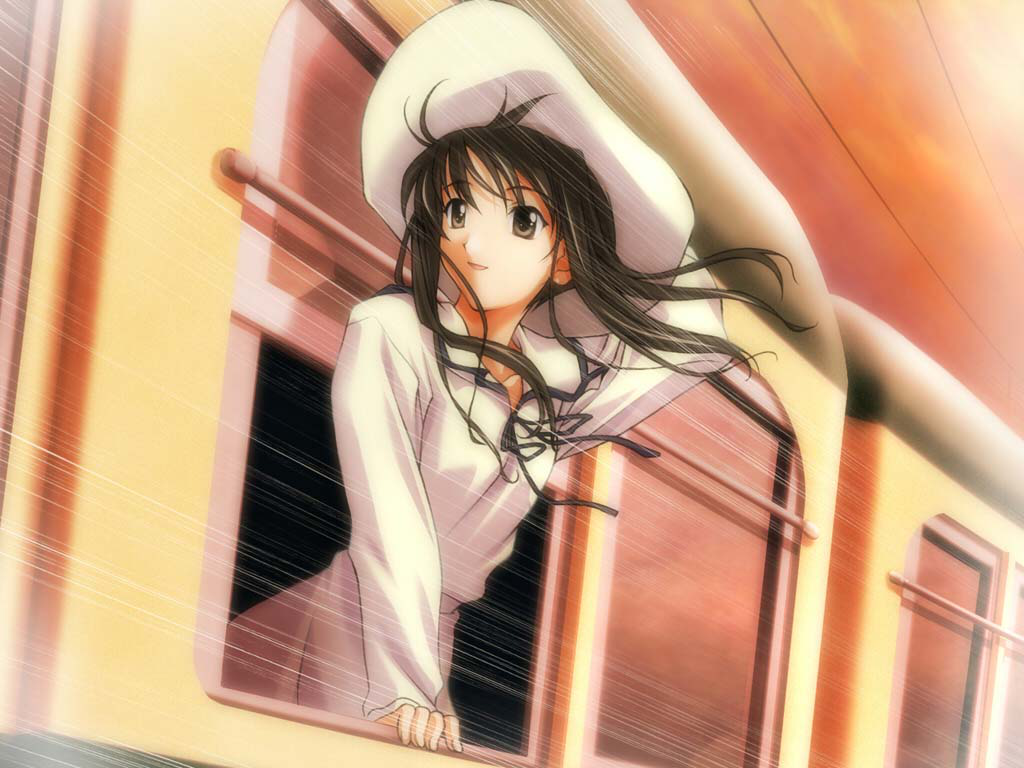
\includegraphics[width=\otherpicwidth]{./res/sample.png}
        }
        \hfil
        \subfloat[南燕]{
            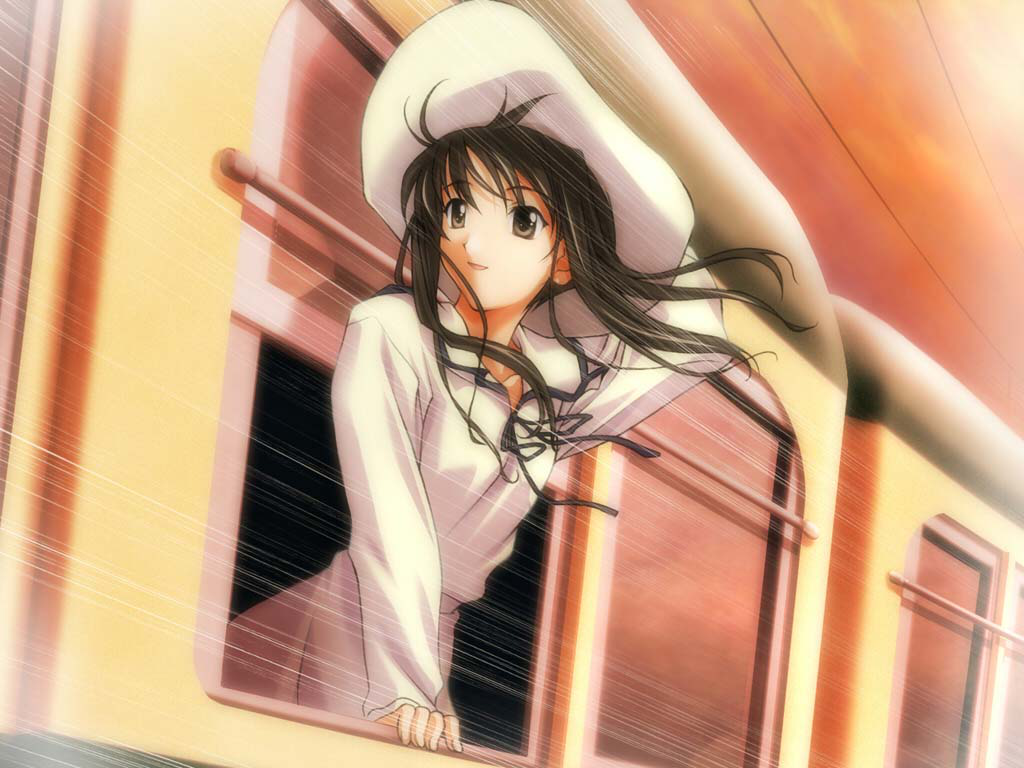
\includegraphics[width=\otherpicwidth]{./res/sample.png}
        }
        \\
        \subfloat[无标题]{
            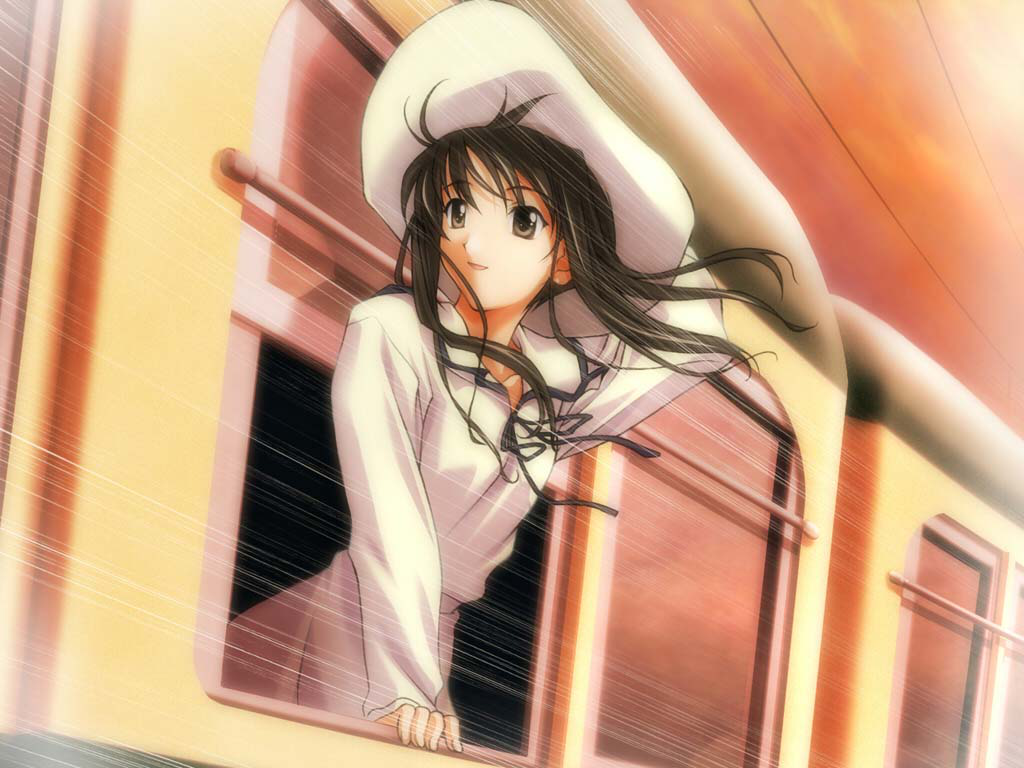
\includegraphics[width=\otherpicwidth]{./res/sample.png}
        }
        \hfil
        \subfloat{
            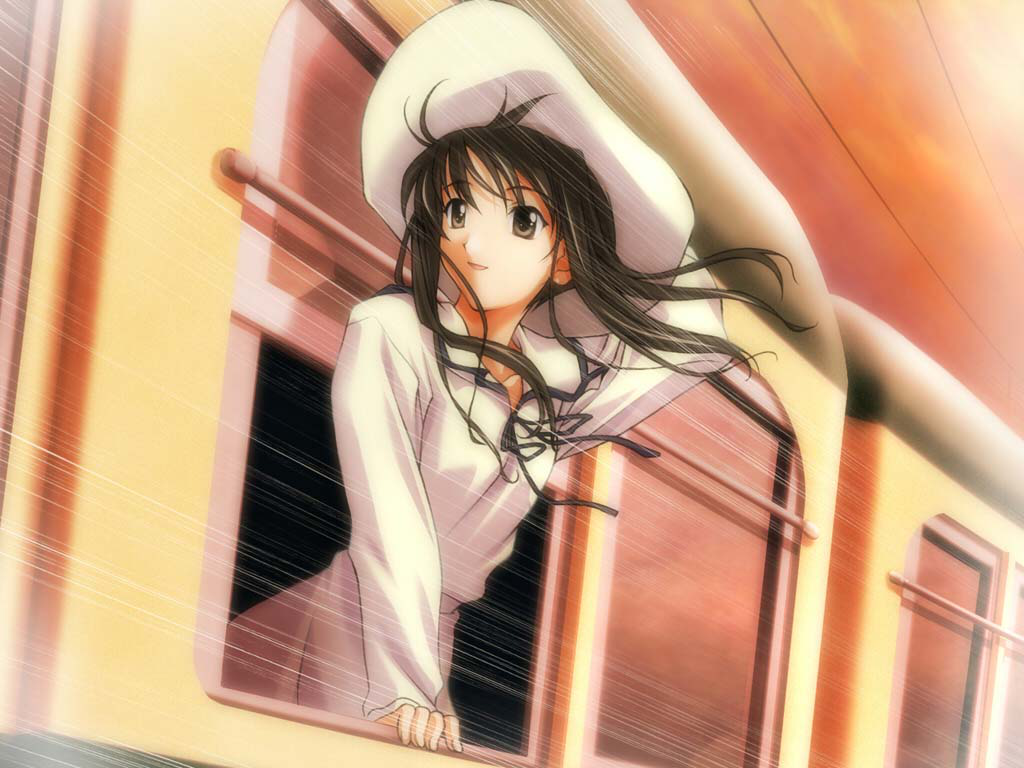
\includegraphics[width=\otherpicwidth]{./res/sample.png}
        }
    \end{figure}
\end{frame}

\subsection{表格}
\begin{frame}
    \begin{table}
    \centering
    \begin{tabular}{lll}
    \hline
    \multirow{2}{*}{\centering  雷达}  &  赛英  &  毫米波雷达样机  \\
    & 北理 & 不详 \\
    \hline
    \multirow{3}{*}{\centering  图像}   &  亿成安  &  分段检测,CCD光学,红外热感应  \\
    & 东信  &  红外热像,云台  \\
    & 旺达世嘉 & 可见光,红外热像仪 \\
    \hline
    \multirow{2}{*}{\centering  二者结合} & 奥普 & 红外辅助照明,微光成像 \\
    & 中电兴发 & 和以色列FODetect系统参数吻合 \\
    \hline
    \end{tabular}
    \end{table}
\end{frame}

\section{常用版式}
\subsection{提示栏}
\begin{frame}{我是标题}
    我是内容
\end{frame}

\subsection{块}
\begin{frame}
    \begin{block}{block}
        content
    \end{block}
    
    \begin{alertblock}{alertblock}
        content
    \end{alertblock}

    \begin{exampleblock}{exampleblock}
        content
    \end{exampleblock}
\end{frame}

\subsection{描述列表}
\begin{frame}
    \begin{itemize}
        \item itemize 1
        \item itemize 2
    \end{itemize}

    \begin{enumerate}
        \item enumerate 1
        \item enumerate 2
    \end{enumerate}

    \begin{description}
        \item[description] details 1
        \item[description] details 2
    \end{description}
\end{frame}

\subsection{上下布局}
\begin{frame}
    \begin{block}{基本思路}
        该处理方法是区域分割方式之一,把图像的坡度看作为山和谷,并将谷底里流出的河川以被山包围的区域来分割检查。
    \end{block}

    \begin{figure}
        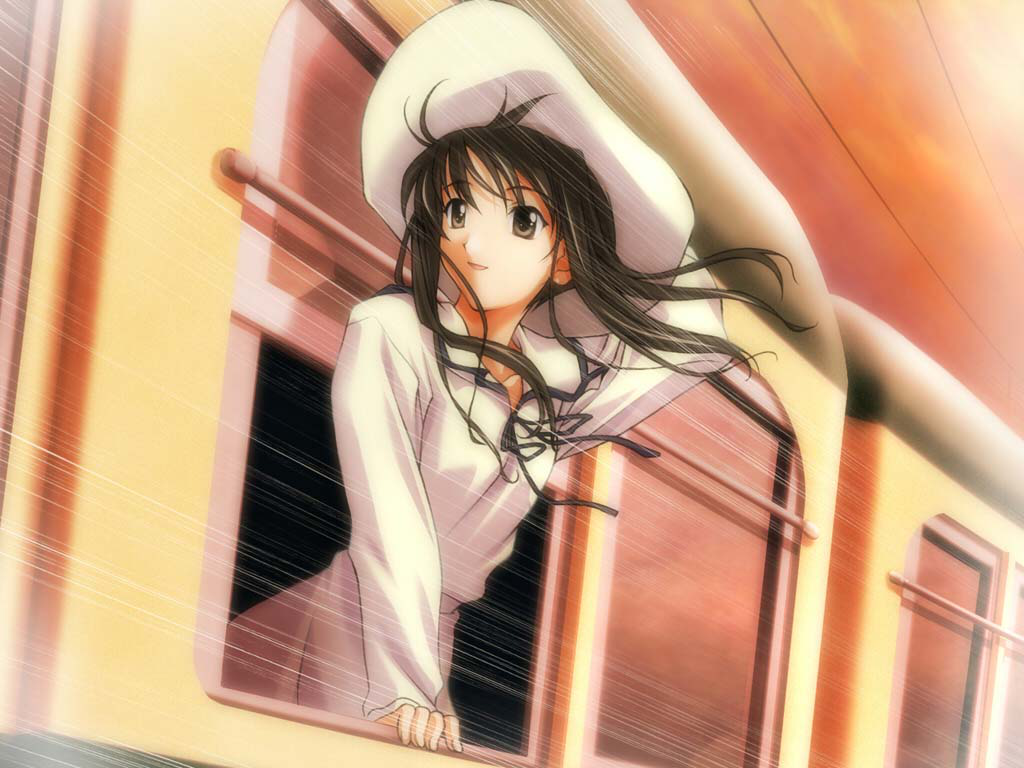
\includegraphics[width=\midpicwidth]{./res/sample.png}
    \end{figure}
\end{frame}

\subsection{左右双栏}
\begin{frame}
    \begin{columns}
        \begin{column}{.3\textwidth}
            \begin{enumerate}
                \item 轮廓提取 
                \item 前景标记
                \item 背景标记
            \end{enumerate}
        \end{column}

        \begin{column}{.6\textwidth}
            \begin{figure}
                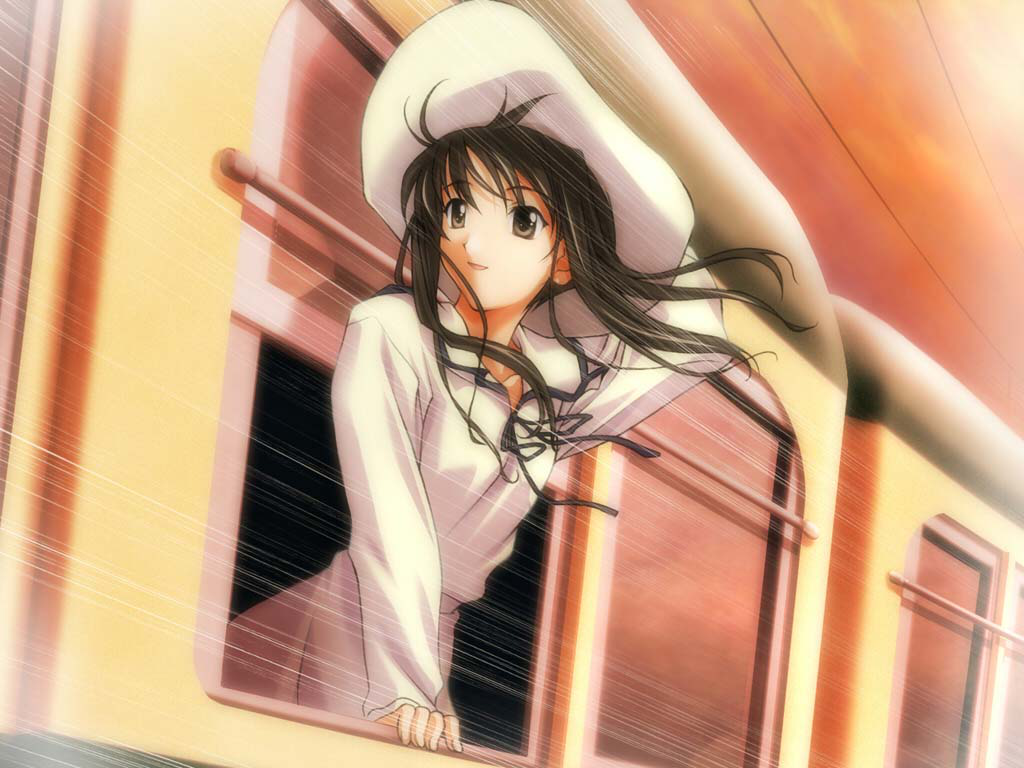
\includegraphics[width=\midpicwidth]{./res/sample.png}
                \caption{女神}
            \end{figure}
        \end{column}
    \end{columns}
\end{frame}

\section{高级}
\subsection{绘图}
\begin{frame}{框架图}
    \begin{figure}[!tb]
        \centering
        \resizebox{\textwidth}{!}{
            \begin{tikzpicture}
                \path (-1,0) node[rectangle, draw](mis) {Mission}
                      (3,0) node[rectangle, color=magenta, draw](dip) {Digital Image Process}
                      (-1,-2) node[rectangle, draw](res) {Resource}
                      (2,-2) node[rectangle, draw](mov) {Move}
                      (4,-2) node[rectangle, draw, red](aut) {Auto}
                      (6,-2) node[rectangle, draw, green](vid) {Video}
                      (2,-3) node[rectangle, draw](mot) {Motor}
                      (4,-3) node[rectangle, draw, green](len) {Lens}
                      (6,-3) node[rectangle, draw](cam) {Camera}
                      (2,2) node[rectangle, draw](net) {Network}
                      (8,1) node[rectangle, draw](dis) {Display}
                      (8,2) node[rectangle, draw, green](key) {Keyboard};
                \draw[thick, <->, >=latex'] (mis.east) -- (dip.west);
                \draw[thick, <->, >=latex'] (mis.south) -- (res.north);
                \draw[thick, <->, >=latex'] (res.east) -- (mov.west);
                \draw[thick, <-, >=latex'] (mov.east) -- (aut.west);
                \draw[thick, ->, >=latex'] (mov.south) -- (mot.north);
                \draw[thick, <-, >=latex'] (aut.east) -- (vid.west);
                \draw[thick, ->, >=latex'] (aut.south) -- (len.north);
                \draw[thick, <-, >=latex'] (vid.south) -- (cam.north);
                \draw[thick, <->, >=latex'] (mis.north) |- (net.west);

                \draw[thick, dashed, <->, >=latex',] (net.east) -- (key.west);
                \draw[] (3.7,2.5) node {TCP};
                \draw[thick, dashed, ->, >=latex',] (vid.east) -| (dis.south);
                \draw[] (8,-2.5) node {UDP};

                \draw[color=gray] (-2.1, 0.5) rectangle (0.1,-2.5);
                \draw[color=gray] (-1,-2.8) node {Control};

                \draw[color=gray] (1, -1) rectangle (7.3,-3.8);
                \draw[color=gray] (2,-4) node {Detector};

                \draw[color=gray] (6.8,2.7) rectangle (9.2,0.3);
                \draw[color=gray] (9.8,1) node {I/O};

                \draw[color=gray] (1.2,-1.5) rectangle (2.8,-3.5);
                \draw[color=gray] (2,-1.3) node {Move};

                \draw[color=gray] (3.3,-1.5) rectangle (7,-3.5);
                \draw[color=gray] (4,-1.3) node {Image};

                \draw[dashed] (6,3) |- (10,-0.5);
                \draw (10,-1) node {API};
            \end{tikzpicture}
        }
    \end{figure}
\end{frame}

\subsubsection{流程图}

\section{其它}
\begin{frame}{符号}
    \begin{itemize}
        \item \CheckedBox \  完成
        \item \XBox \  失败 
        \item \Square \  等待
    \end{itemize}
\end{frame}

%---------
\createlastpage

\end{document}

